\section{ESTHETE: A system for context-full news browsing }

In this section we first describe the key features of our system. Next, we give a block design of our system, followed by a detailed explanation
of each component. 

\subsection{Key features of ESTHETE}

\subsubsection{Returning related articles}
Our system returns additional articles which bring out related aspects of the story (subgraph) that the user is studying, and reading which helps
the user get the big picture. The news graph not only tells us the articles related to a particular story (neighbourhood of a subgraph), but
also \emph{qualifies} how these articles are related, by way of the nature of the transformations that the edges cover. For eg., consider a subgraph $S$, with
2 node neighbours $A$ and $B$ shown in Figure~\ref{fig:related-articles}. Say a user is following a news story involving the people $P1$, $P2$ and
$P3$. Clearly, the user's understanding of this story depends on whether she follows these people and their past interactions in other stories.
The graph can figure out that article $A$ is a good \emph{starting} point for the user to understand how $P2$ comes into the story she is
following. Similarly, it can also qualify the importance of article $B$ to the subgraph. Note that the system just suggests these contexts to the user, allowing them to finally decide whether to explore these or not. 
\begin{figure}
\begin{center}
\caption{The news graph qualifies every relation mined in the news corpus}
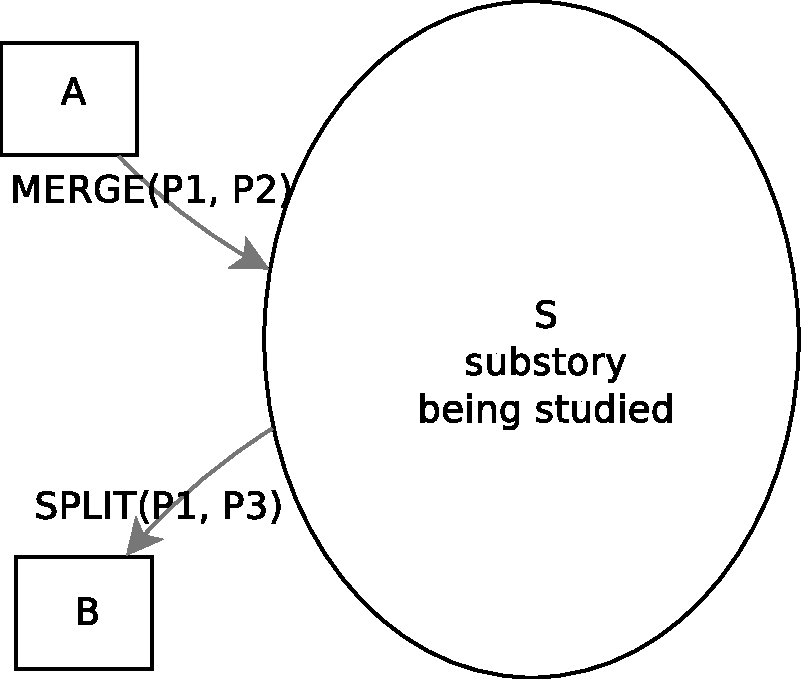
\includegraphics[scale=0.34]{figures/graph-4.pdf}
\label{fig:related-articles}
\end{center}
\end{figure}

\subsubsection{Queryability}
Our system is queryable by users, where a query entered by a user is in the form of filter on the actors and/or topics talked about in the
news corpus. Hence, the users need only to pick a suitable filter to study the intended story in desired detail. For eg., an example query could
be ``CORRUPTION AND ROBERT VADRA AND HARYANA'' which yields all stories around the corruption scandal involving Robert Vadra
(an Indian businessman) in Haryana (a state in India).
\subsubsection{Faceted Searchability}
Our system is a guided environment where a user is presented with popular actors, topics, events, time periods, etc automatically from the 
news corpus, which guide her search to discover and explore more popular stories first. These also serve to label different stories, guide the
user towards a more refined query around specific substories. Figure~\ref{fig:faceted-search} shows a snapshot of this feature.
\begin{figure}[ht]
\begin{center}
\caption{Analytics which help the user better understand the stories}
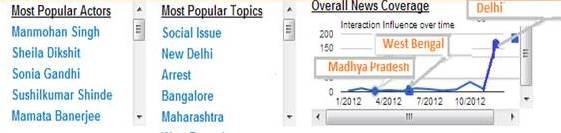
\includegraphics[scale=0.34]{figures/faceted.png}
\label{fig:faceted-search}
\end{center}
\end{figure}

\subsubsection{Structured storage of an article stream}
The rate at which new articles are published is growing exponentially. If a system
has to do well at taking in a live input stream of news articles, it can afford to process this set only once, and then store this set in a structure
which is efficient to maintain and query later. In most cases, this structure would come from the text content of the articles coming from a third-party media organization, 
but once derived, the text content need not be duplicated by the browsing system. The structure should be rich enough to answer all queries of the user, without
processing the article text again.
\subsubsection{On-demand detail}
The system should respect the user's final say in the detail at which different stories are visualized. Should the system
just give a 10-line summary of the event captured by 5 articles? Or should it focus in to the 5 articles, creating 2 sub-stories within them? This decision
should be left to the user as a preference.
\subsubsection{No Redundancy in the News stories}
News articles around a single story tend to summarize past events, so as to be give some 
context to the reader following this story. However, a browsing system should remove such redundancy, and summarize various facets of the story
that are developed in the sequence of articles, so as event appears once at the time of first reporting
\subsection{Block System Design}
\label{sec:block}

The strength of our approach is that we only need to process our input news article set only once. From the raw set of news articles, we
generate and store a graph representation formed by considering the most important transformations that are mined. We claim that this graphical 
representation of the article set is rich enough to answer different kinds of user queries. Having created a news graph from the news corpus, we showed how to meet the requirements of a good news browsing system.
Figure~\ref{fig:block-system-design} shows our block system design. It can be divided into
two major components - Offline and Online. The offline component handles incoming news articles, and augments them into our underlying graph data structure representation stored
in the database. The online component interfaces with the user, and based on the user's query, identifies the parts of the graph to visualize and 
shows the relevant stories. To further save, we need only save the structure with pointers to web URL of the article to be queried only while presenting to the user. We will now briefly describe each aspect of our system.
\subsection{Preprocessing Steps}
\subsubsection*{News Corpus}
Our news corpus is a subset of articles from the Indian national daily {\em The Hindu}\footnote{http://thehindu.com}, across a variety of broad categories like Crime, Economy, Government, etc. 
{\em The Hindu} was chosen because it is a popular Indian daily, and offers a convenient way to download articles along with rich meta-data like Topic tags.
\subsubsection*{Entity Extraction}
We used the OpenCalais\footnote{http://opencalais.com} API to extract all the entities appearing in the articles. In particular, we call
the people featured in the articles as actors. We found the result of OpenCalais to be the most accurate among the NER tools we experimented with.
For sanitizing the mined entity set (correct spelling errors, remap aliases of the same entity to a unique identifier, remove ambiguous entity tokens),
we used an ontology(YAGO\footnote{http://www.mpi-inf.mpg.de/yago-naga/yago/}) based approach.
\subsubsection*{Topic Detection}
Along with the entities for an article, we also need the list of topics that were talked about in the article. 
We relied on the Hindu articles being hand tagged-at-source by rich and relevant Topic tags. These are much more expressive compared to an automated technique of topic detection.
\begin{figure}
\caption{Block system diagram of our News Browsing tool}
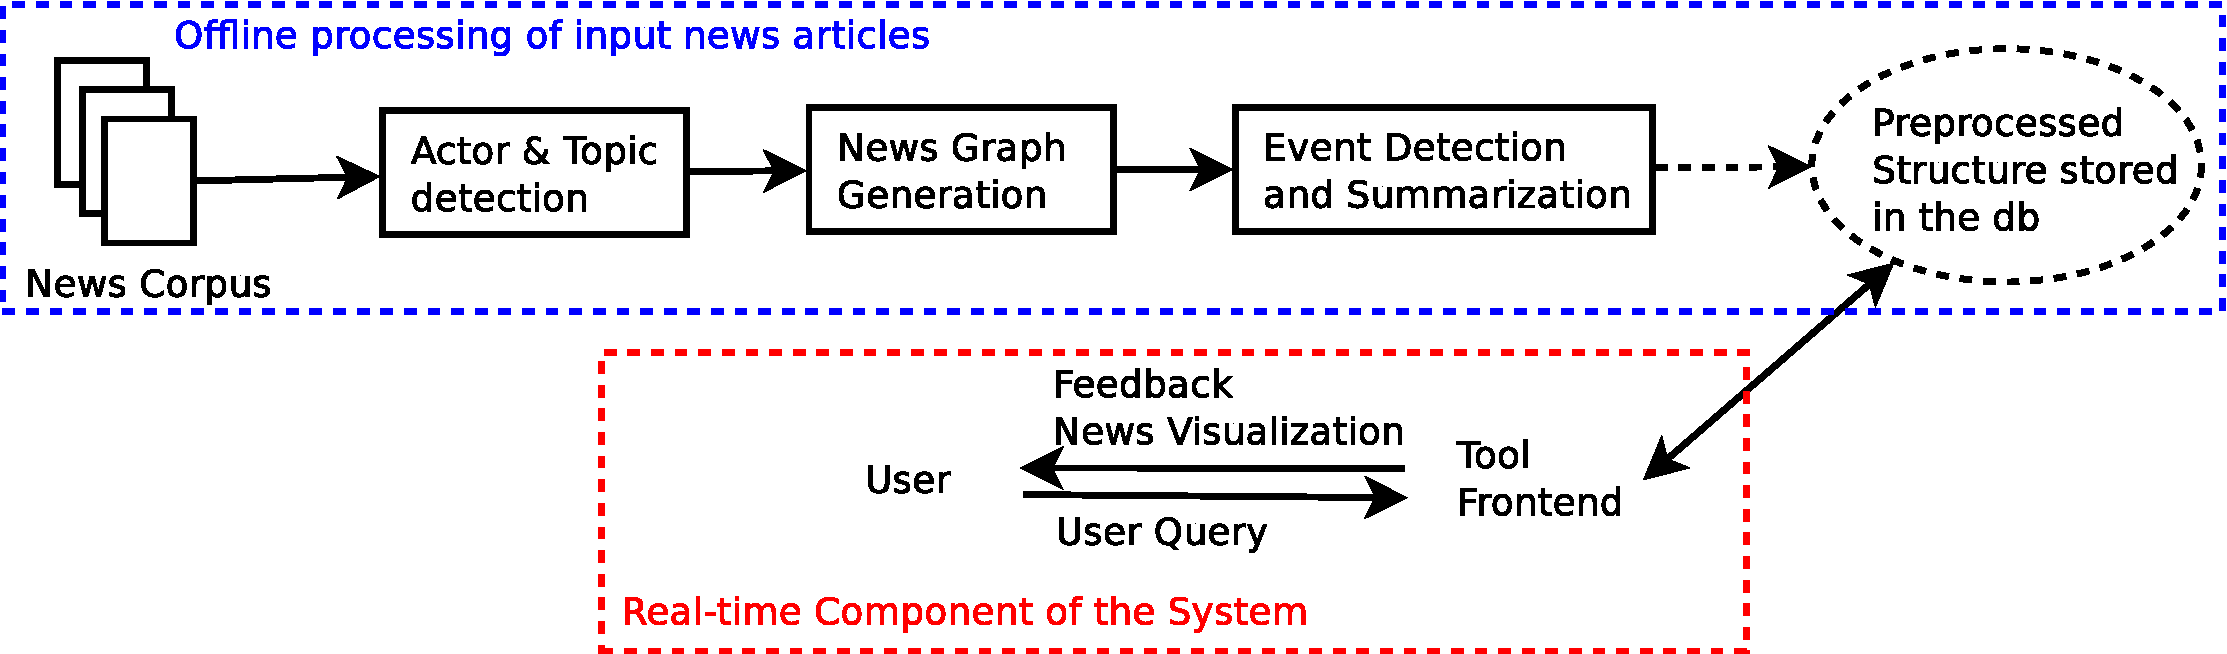
\includegraphics[scale=0.24]{figures/system-design.pdf}
\label{fig:block-system-design}
\end{figure}
\begin{figure*}
\caption{A graph snippet showing multiple stories}
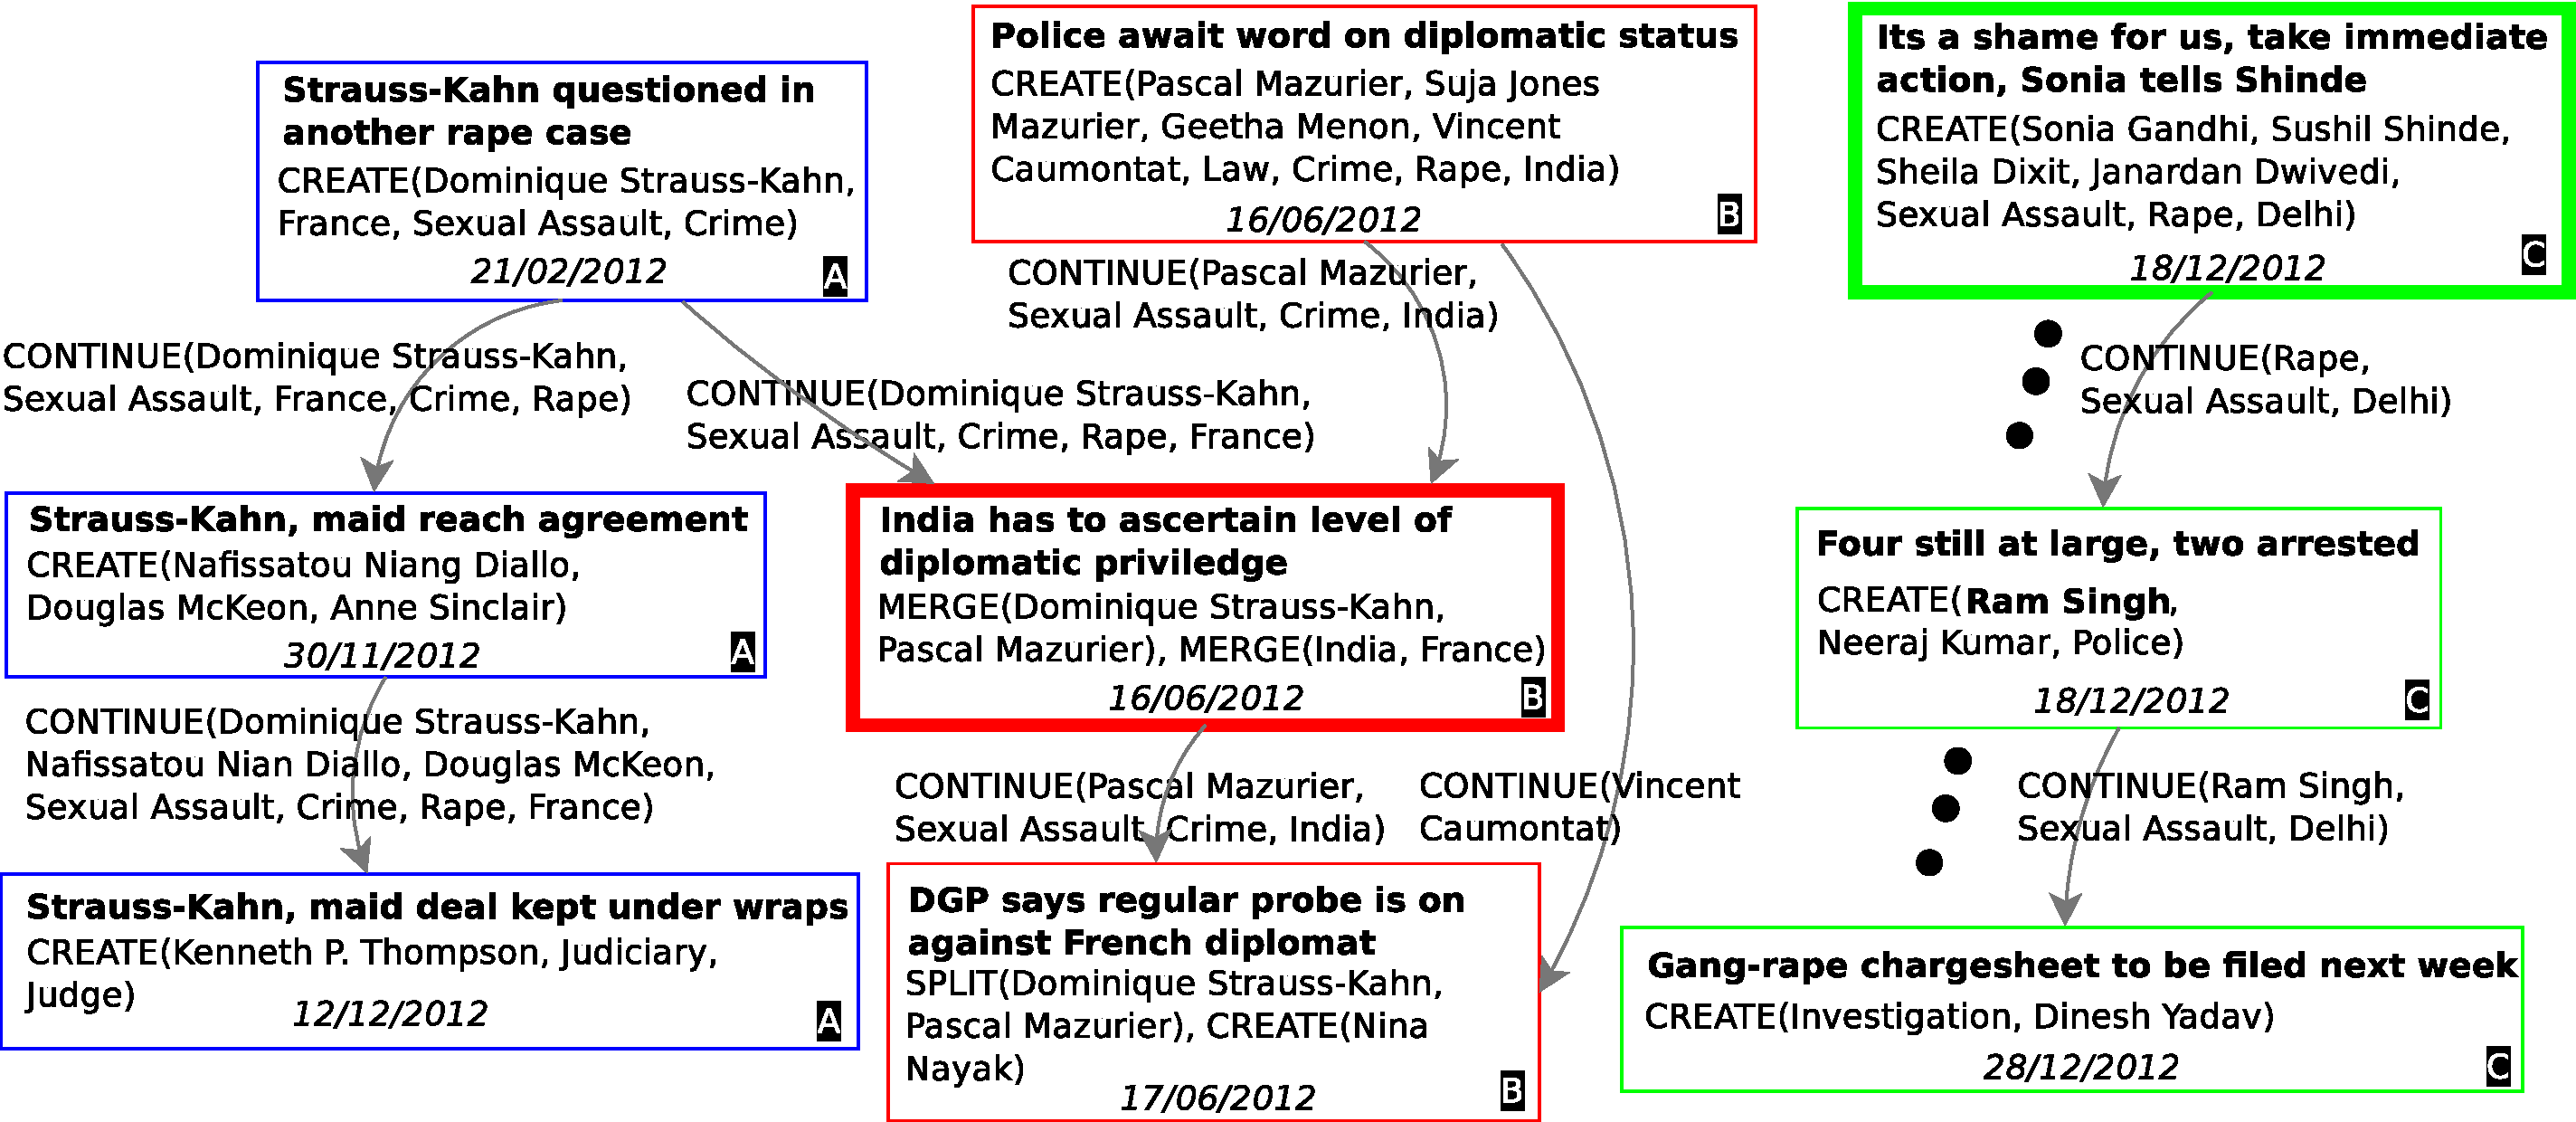
\includegraphics[scale=0.34]{figures/graph-2.pdf}
\label{fig:context-graph-example}
\end{figure*}

\subsection{News Graph Generation}\label{sec:graph-desc}
Our work implements and builds upon the work by Choudhary et
al.\cite{choudhary@ecir2008} which formalizes the notion of presenting
news articles as a directed graph.  Their algorithm can be extended to
augment new articles on to a pre-built graph since it considers
articles sequentially.  The following sequence of update steps are to
be followed on augmenting a new article $a_t$ published at $t$, into
the graph structure.
\begin{enumerate}
  \item Tag $a_t$ with relevant actors and topics
  \item Find all articles $A = a_\tau$ s.t. $\tau+F \leq t$.
  \item For the articles in the set $A$, mine all additional transformations that emerge
  \item Recompute the min-weight edge-covering locally in the subgraphs containing articles from $A$
  \item For the new article $a_t$, repeat the steps required for adding a new article into the graph
  \item Re-cluster the graph locally to determine to assign a cluster to the new node
\end{enumerate}
By taking the recommended values of the parameters, we were able to generate a news graph on 1000 nodes in around 4 minutes on a Dell Intel Centrino machine.
Adding newer articles to this graph was significantly cheaper, taking only around 10 seconds depending on the article size, etc.
Moreover, it only looks at articles within a time window, and hence different parts of the graph can be generated in parallel.

Figure~\ref{fig:sample-news-graph}  shows an example a part of the graph created on articles that followed a Rape Case incident during February-April 2012. We see how the
story starts with the media covering initial case being filed and the police investigations.

\subsection{Event detection, summarization \& Context extraction}\label{sec:event-detection-summary-context}
\subsubsection*{Event detection}
We found the resultant graph from the previous step not suitable for visualization. The graph created is usally very dense, making it hard to follow and study a subgraph in isolation.
Every edge in the graph covers some transformations between articles, however to convey the purpose of every edge, one needs to label it with the transformations that the edge covers, 
which further makes visualization overwhelming. 
We consider this graph more suitable as a rich back-end.
This graph is created by pre-processing the news corpus once, and then a standard node clustering algorithm (Markov graph clustering) is applied to draw out clusters in this graph. 
These clusters are considered as events that happen in the corpus. Different clusters may or may not talk about the same story, depending on the proximity of the clusters.
In this way, an event is a cluster of the news graph, which may contain one or more articles. 
This graph is now useful for answering questions like detecting significant events (dense node clusters), developments in the life of a particular group of actors (visualizing the subgraphs 
involving the actor set), etc. The intuition behind how the graph structure relates to events in the real world is natural if we study how media reports events. 
For eg., consider an event like some criminal offence followed by a law suite. At first, articles start appearing which talk about the offence and alleged victims and culprits. Then, this is gradually
replaced by the ongoing trial. Across these articles, the common threads are the topics and the CONTINUE/MERGE transformations among the actors (victims and culprits). Hence, these naturally form node clusters in the graph. This real world event is captured 
by the sequence of the articles that appeared.
As we show in Section~\ref{sec:baseline-comparison}, events determined by way of clustering on the graph is preferred by users to a similar clustering
done on raw articles in most cases.
\subsubsection*{Event summarization}
To make it easier for the user to understand an event, we summarize the articles part of this event to give a broad idea of the event and show this summarization alongside the articles capturing that event (Section \ref{sec:filter-summarization}). For this, we tried out various document summarizing tools. We finally decided to Text Compactor \footnote{http://textcompactor.com/} which is based on Open Text Summarizer\footnote{http:/libots.sourceforge.net/} and has a convenient API. 
\subsubsection*{Context extraction}
Due to richness of the news graph, the neighbourhood of the story (subgraphs of the base news graph) being currently visualized, serves to add
useful context. Moreover, different parts of the neighbourhood model different transformations and hence, following
different neighbours amounts to adding a more unique kind of context, which gives a unique interpretation of the overall story. 
\subsection {Frontend interface}
Our interface is built on HTML using Javascript and PHP on the server-side, using TimelineJS\footnote{http://timeline.verite.co/} and Google Visualization API\footnote{http://developers.google.com/chart/interactive/docs/reference} libraries.
Figure~\ref{fig:complete-tool-screenshot} shows a screenshot of our webtool. The interface
has 3 primary parts: the Filtering \& feedback pane, the News article(s) \& summary pane and the Timeline pane. 
\subsubsection*{Filtering \& feedback pane}
Our system deeply analyzes the news corpus to mine all the featured actors and topics, and makes them queryable. The user selects one or more actors
and/or topics to filter news only about them. The user could also restrict on a particular time window. Relative to the filter parameters set by her, 
the user gets more context by way of getting a ranked list of ``Popular Actors'' and ``Popular Topics''. In addition, we also plot the number of
articles published against time to study what stories were popular at what times. 
\subsubsection*{Timeline pane}
Having selected suitable filters, the user is presented with all the different events detected from the graph on the timeline. These appear as 
bubbles on the timeline, with a start and end date. The user can easily move in time, skimming through uninteresting news events.
More popular events (as judged by the density of nodes \& edges in the cluster), are highlighted in yellow to guide the user.
On clicking a particular bubble, that event is highlighted and the corresponding story is shown in the middle pane. Figure~\ref{fig:timeline-closeup}
shows a snippet of the timeline, with each bubble an event (one or more articles) at some time, and the most significant bubble highlighted in yellow.
\begin{figure}
\caption{A screenshot of the timeline showing event bubbles}
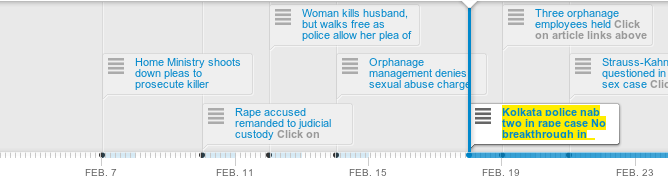
\includegraphics[scale=0.34]{figures/timeline2.png}
\label{fig:timeline-closeup}
\end{figure}
\subsubsection*{News articles \& summary pane}\label{sec:filter-summarization}
Having selected a particular story to focus on, the user can read all articles arranged sequentially so it is easy to read them in succession.
On the right, we show a summary generated from the articles of this story by the methods discussed in Section \ref{sec:event-detection-summary-context}.
On clicking an article, the user is served the full article text. The user is also shown the full list of actors and topics discussed in this story.
